% Preamble
\documentclass[a4paper, 12pt]{article}
\usepackage[margin=1in]{geometry} % Set margin
\usepackage{pdfpages} % Insert pdf pages
\usepackage{amssymb,amsmath,amsthm, amsfonts} % Math libraries

% Custom commands
\newcommand{\sub}[1]{\subsection{\underline{#1}}}
\newcommand{\subsub}[1]{\subsubsection{\underline{#1}}}
\newcommand{\R}{\ensuremath{\mathbb{R}}}
\newcommand{\F}{\ensuremath{\mathbb{F}}}
\newcommand{\N}{\ensuremath{\mathbb{N}}}
\newcommand{\Onef}{\ensuremath{1_{\F}}}
\newcommand{\Zerof}{\ensuremath{0_{\F}}}
\newcommand{\eqbcuz}[1]{\text{~$\stackrel{(#1)}{=}$~}}
\newcommand{\eq}[1]{\begin{align*}#1\end{align*}}
\newcommand{\eqn}[1]{\begin{align}#1\end{align}}
\newcommand{\set}[1]{\big{\{} #1 \big{\}}}
\newcommand{\bigset}[1]{\bigg{\{} #1 \bigg{\}}}
\renewcommand{\qed}{\hfill\(\qedsymbol\)}
\newtheorem{lemma}{Lemma}

% Begin Document %
\begin{document}

% Title Page
\begin{titlepage}
    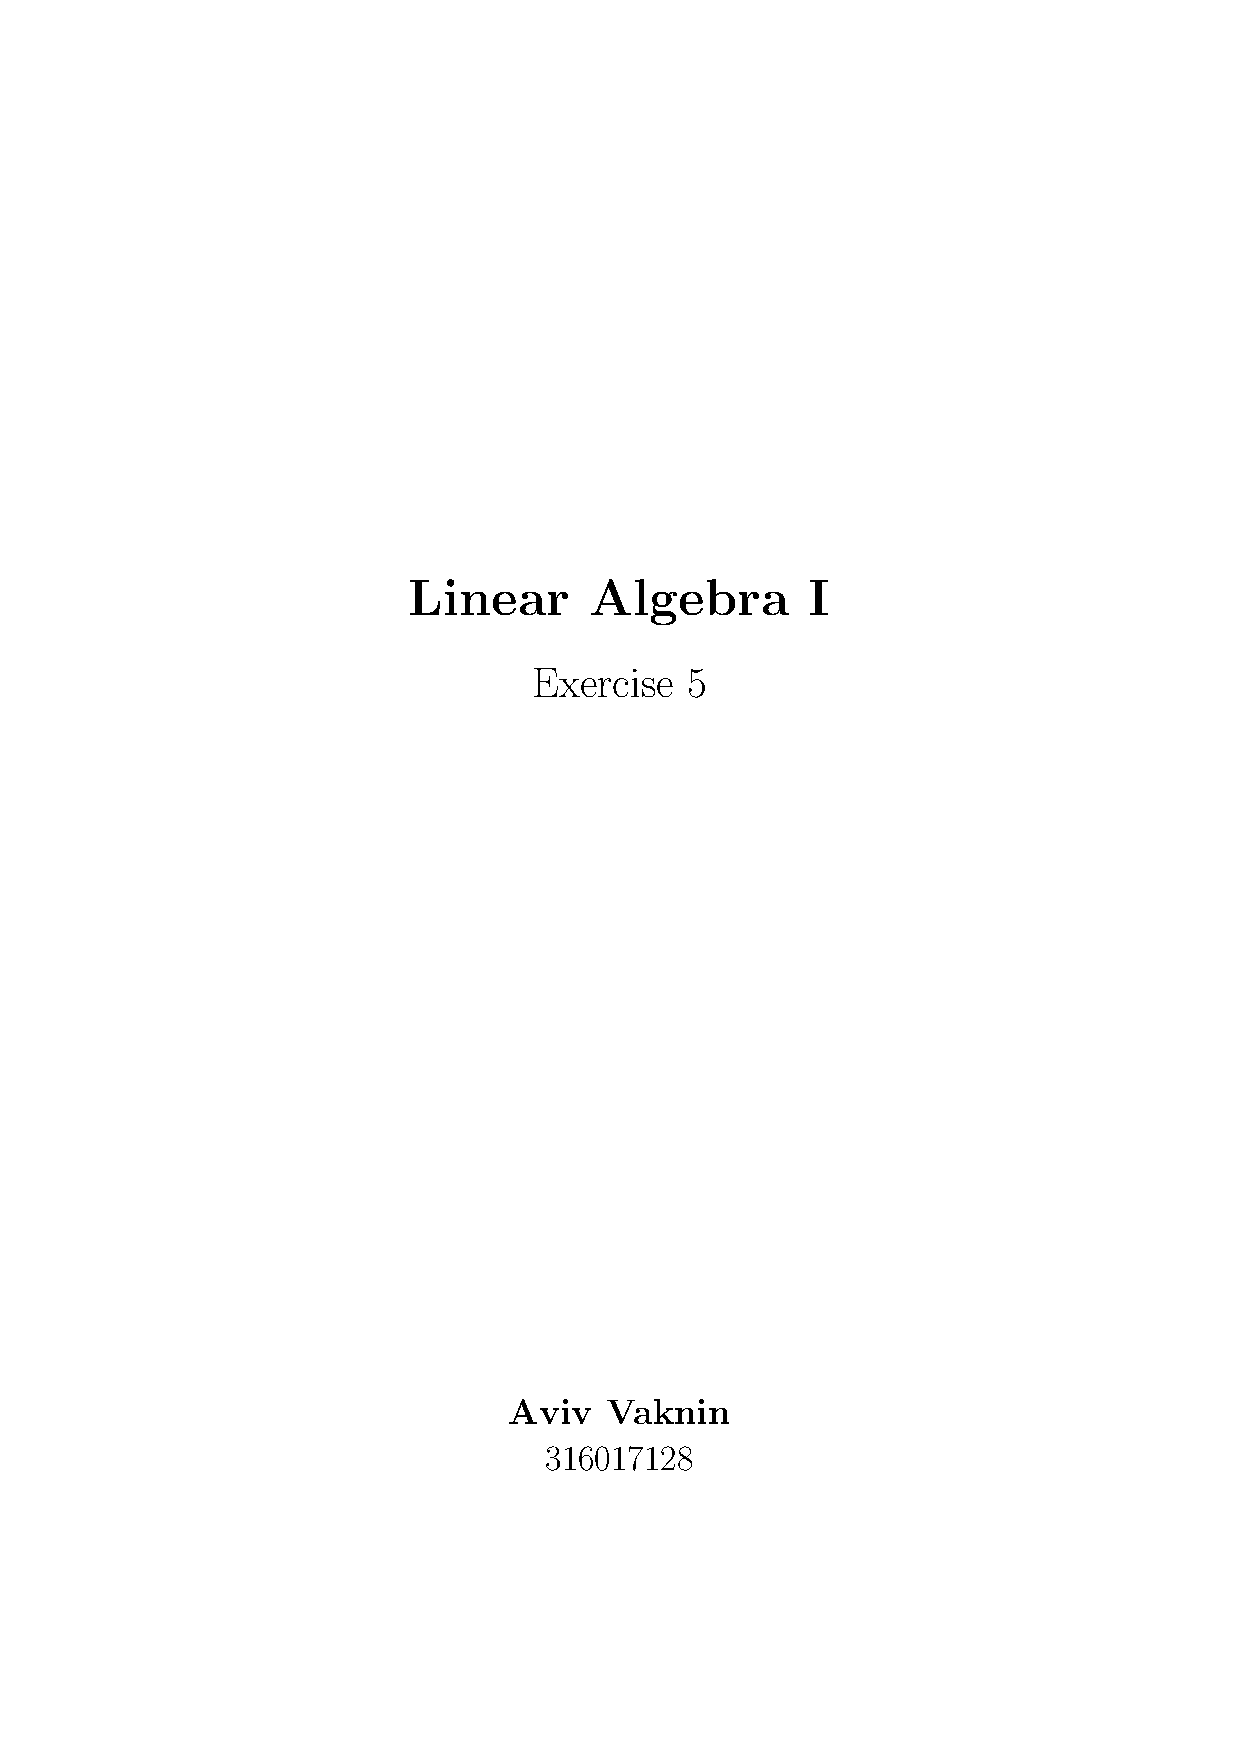
\includepdf{title.pdf}
\end{titlepage}

% 2
\setcounter{section}{1}
\section{}
\sub{Calculate $A^2, B^2, AB$ and $BA$}
\eq{
    A^2=\begin{bmatrix}
        1&2&1&0&0\\
        0&1&2&0&0\\
        0&0&1&0&0\\
        0&0&0&1&2\\
        0&0&0&0&1
    \end{bmatrix}
}
\eq{
    B^2=\begin{bmatrix}
        1&0&2&0&0\\
        0&1&0&0&0\\
        0&0&1&0&0\\
        0&0&0&-1&0\\
        0&0&0&0&-1
    \end{bmatrix}
}
\eq{
    AB=\begin{bmatrix}
        1&1&1&0&0\\
        0&1&1&0&0\\
        0&0&1&0&0\\
        0&0&0&1&-1\\
        0&0&0&1&0
    \end{bmatrix}
}
\eq{
    BA=\begin{bmatrix}
        1&1&1&0&0\\
        0&1&1&0&0\\
        0&0&1&0&0\\
        0&0&0&0&-1\\
        0&0&0&1&1
    \end{bmatrix}
}
\eq{
    A^k=\begin{bmatrix}
        1&k&(A^{k-1}+(k-1))&0&0\\
        0&1&k&0&0\\
        0&0&1&0&0\\
        0&0&0&1&k\\
        0&0&0&0&1
    \end{bmatrix}
}
\eq{
    B^k=\begin{bmatrix}
        1&0&k&0&0\\
        0&1&0&0&0\\
        0&0&1&0&0\\
        0&0&0&x&y\\
        0&0&0&z&w
    \end{bmatrix}
}
When $x,y,z$ and $w$ alternate between $-1, 0$ and $1$.

% End Document %
\end{document}